\documentclass{article}

\usepackage{url} 

\usepackage{pdfpages}
\usepackage{lastpage}
\usepackage{fancyhdr}
\usepackage{ngerman}
\usepackage{listings}

\usepackage{floatrow}
\usepackage[tableposition=top]{caption}
\floatsetup[table]{capposition=top}

\usepackage{amsmath, amssymb}

\usepackage[utf8]{inputenc}


\usepackage[numbib]{tocbibind}



\newcommand\twodigits[1]{%
   \ifnum#1<10 0#1\else #1\fi
}



\lhead{Oszillograph}
\rhead{16. Oktober 2020\\T. Maier, J. Winkler}
%\cfoot{\twodigits{\thepage}~/ \pageref{LastPage}}
\cfoot{{\thepage}~/ \pageref{LastPage}}

\newcommand{\as}{\alpha_\text{spez}}

\begin{document}

\parindent0cm

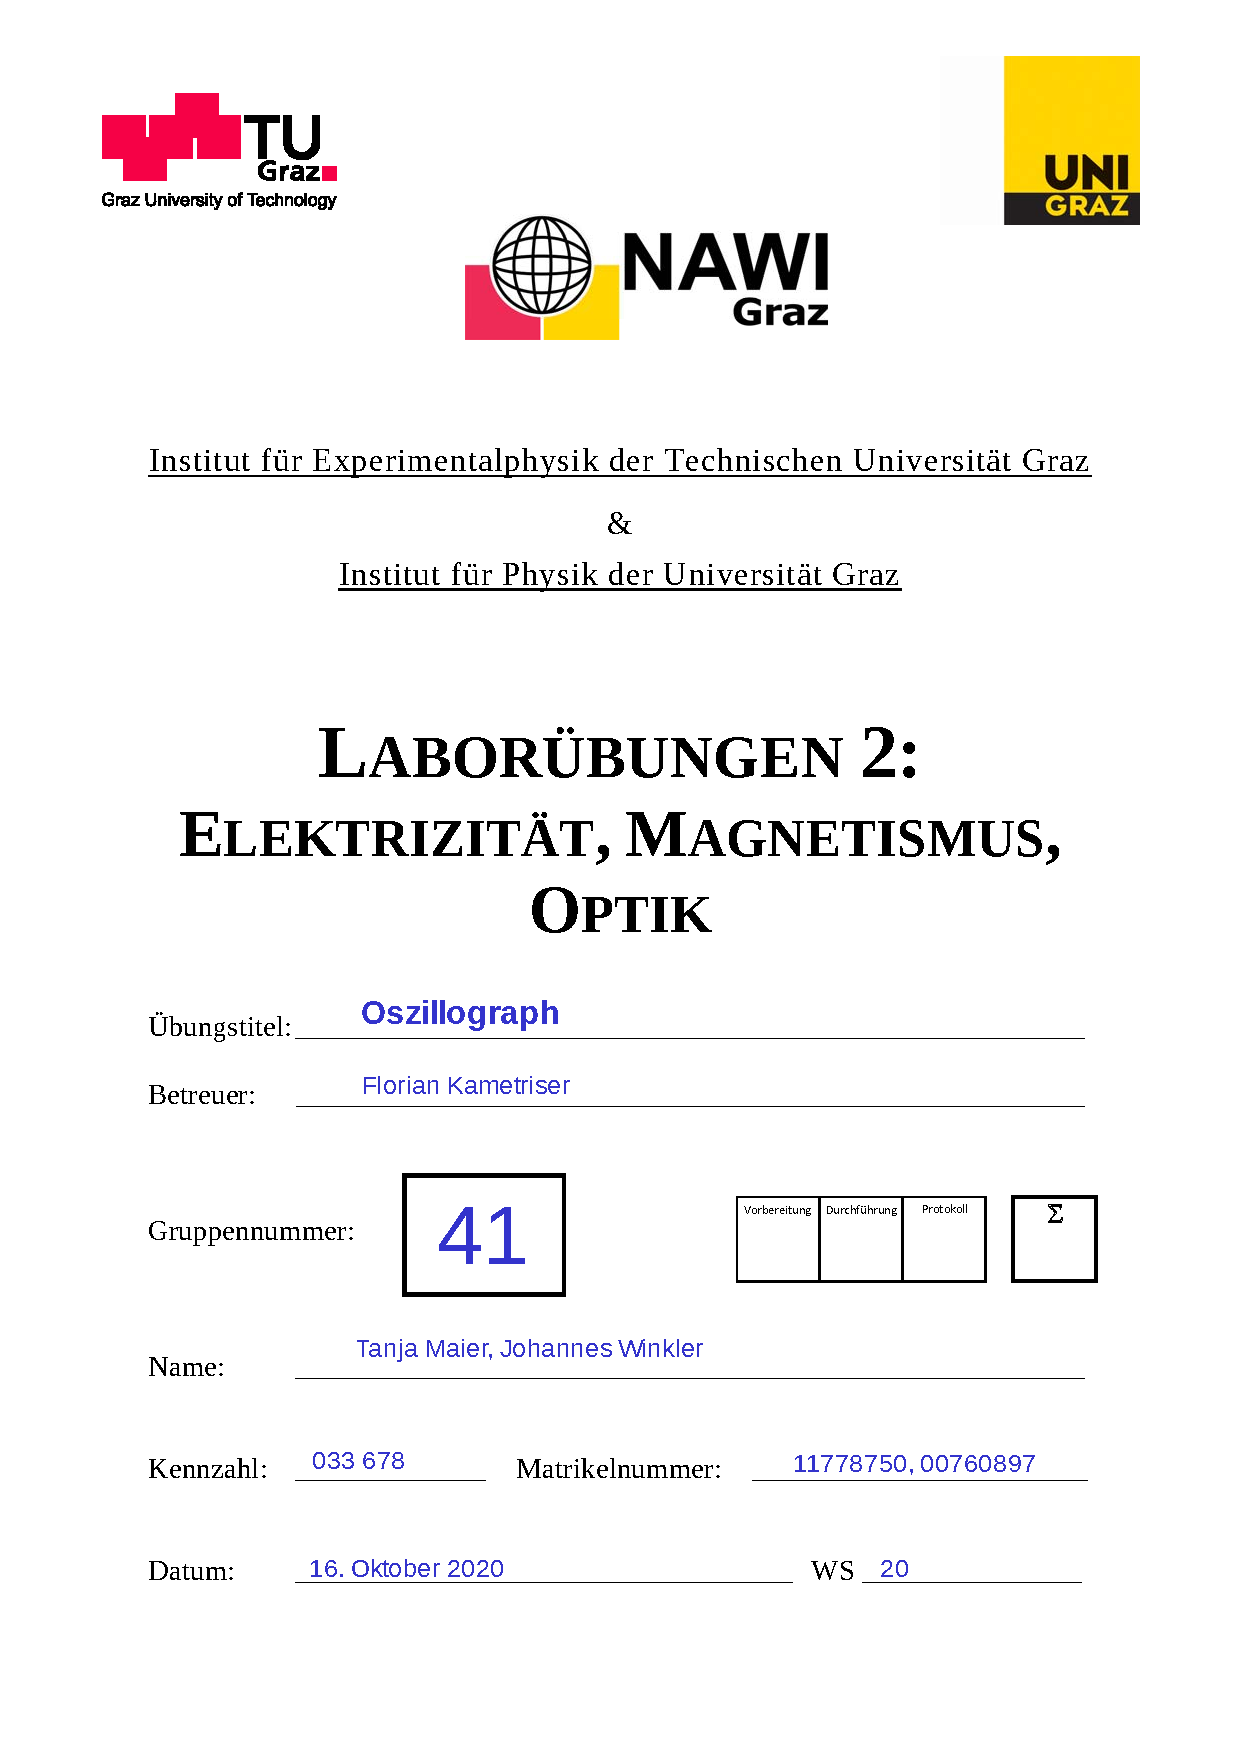
\includepdf{Deckblatt.pdf}


\pagestyle{fancy}

\section{Aufgabenstellung}


\section{Grundlagen und Versuchsaufbau}

\subsection{Oszilloskop}

Ein Oszilloskop ist ein Gerät aus der Elektronik, mit dem man Spannungsschwankungen innerhalb zeitlicher Abläufe messen kann. Auf der $x$-Achse ist dabei die Zeit und auf der $y$-Achse die jeweilige Spannung abzulesen.

Das Prinzip dahinter ist auf die Bewegung von Teilchen in einem elektrischen Feld und somit auf die Braun'sche Röhre zurückzuführen.

Bei der Braun'schen Röhre (= Kathodenstrahlröhre) kann durch zwei parallel ausgerichtete Metallplatten Elektronenstrahl quer zu seiner Flugrichtung beeinflusst werden. Die Elektronen werden von der Kathode emittiert und durch eine angelegte Spannung zur Anode $A$ hin beschleunigt.

Um den Strahl zu fokussieren werden zwei elektrische Linse $F$ und die angelegte Fokussierspannung $U_F$ genutzt.


Zur Ablenkung des Elektronenstrahls werden dann vier weitere Platten nach der Anode angebracht. Diese werden zu zweit platziert und mit einer horizontalen Kippspannung ($U_x$) bzw. einer vertikalen Messspannung ($U_y$) versehen. Damit werden die Elektronen abgelenkt und treffen auf den Leuchtschirm am Ende der Röhre.

Mithilfe der Spannung zwischen Kathode K und Wehnelt-Zylinder WZ kann dann noch die Helligkeit des am Schirm abgebildeten Leuchtpunktes variiert werden. \cite{braun} \cite{uniunterlagen}

\subsection{RLC-Stromkreis}

Ein RLC-Stromkreis besteht aus einem Kondensator mit der Kapazität $C$, einer Spule mit Induktivität $L$ und einem Widerstand mit der Größe $R$. Alle Bauteile sind hierfür in Reihe geschalten und somit gilt die Kirchhoff'sche Maschenregel
\begin{align}
\label{eq:maschen}
U_C + U_L + U_R = 0
\end{align}

$U_C$ ist dabei die Spannung am Kondensator, $u_L$ die Spannung an der Spule und $u_R$ die Spannung am Widerstand. Durch Ersetzen von 
\begin{align*}
U_L &= L \cdot \frac{dI}{dt} \\
U_R &= R_i \cdot I
\end{align*}
sowie differenzieren der Formel \eqref{eq:maschen} und ersetzen von 
\begin{align*}
I = i_C = C \cdot \frac{dU}{dt}
\end{align*}
 erhält man die Differentialgleichung des Schwingkreises
\begin{align}
\frac{d^2I}{dt^2} + \frac{R}{L}\cdot \frac{dI}{dt} + \frac{1}{L\cdot C}\cdot I = 0
\end{align}
Durch Lösung dieser Differentialgleichng ergeben sich im wesentlichen 3 mögliche Fälle
\begin{enumerate}
\item $R^2\cdot C - 4\cdot L > 0$: 2 Reelle Lösungen, Kriechfall
\item $R^2\cdot C - 4\cdot L = 0$: 1 reelle Lösung, aperiodischer Grenzfall
\item $R^2\cdot C - 4\cdot L < 0$: 2 konjugiert-komplexe Lösung, Schwingfall
\end{enumerate}




\section{Geräteliste}

\begin{table}[H]
\caption{Liste der verwendeten Geräte}

~

\begin{tabular}{l|llll}
Bezeichnung & Hersteller & Gerätenummer & Unsicherheit \\
\hline
Frequenzgenerator & Wavetek & 0161674  \\
Trafo & \\
Oszilloskop & RIGOL &DS1ET204711289 \\
Widerstand $1$~k$\Omega$ & Rosenthal & & $\pm~1\%$ \\
Widerstand $200~\Omega$ & Rosenthal & & $\pm~1\%$ \\
Spule $n=500$ & & 843/3 \\
Kondensator $1~\mu$F & Philips
\end{tabular}

\end{table}




\section{Durchführung und Messwerte}


\section{Auswertung}




\section{Zusammenfassung und Diskussion}



%\newpage 
%\appendix
%\section{Python Skript}



\definecolor{commentgreen}{RGB}{2,112,10}
\definecolor{eminence}{RGB}{108,48,130}
\definecolor{weborange}{RGB}{255,165,0}
\definecolor{frenchplum}{RGB}{129,20,83}

\lstdefinelanguage{python}{
    morekeywords={def, for, range, abs, return},
    otherkeywords={<-,->, |>, \%\{, \}, \{, \, (, )},
    sensitive=true,
    morecomment=[l]{\#},
    morecomment=[n]{/*}{*/},
    morecomment=[s][\color{purple}]{:}{\ },
    morestring=[s][\color{orange}]"",
    commentstyle=\color{commentgreen},
    keywordstyle=\color{eminence},
    stringstyle=\color{red},
	basicstyle=\ttfamily,
	breaklines,
	showstringspaces=false,
	frame=tb
}
%\lstinputlisting[language=Python,captionpos=b, label=lst:test,caption={Laplace Auswertung}]{generate_numbers_laplace.py}

%\lstinputlisting[language=Python,captionpos=b, label=lst:test,caption={Bessel Auswertung}]{generate_numbers_bessel.py}


%\lstinputlisting[language=Python,captionpos=b, label=lst:test,caption={Zerstreuungslinse Auswertung}]{generate_numbers_zerstreuungslinse.py}


\begin{thebibliography}{9}
\bibitem{braun} \url{https://www.leifiphysik.de/elektrizitaetslehre/bewegte-ladungen-feldern/ausblick/braunsche-roehre}
\bibitem{youtube} \url{https://www.youtube.com/watch?v=TZQoyem7Jzo}
\bibitem{signale} \url{https://www.rahner-edu.de/grundlagen/signale-richtig-verstehen/schwingkreise/}
\bibitem{RLC} \url{https://itp.tugraz.at/wiki/index.php/RLC-Serienschwingkreis}
\bibitem{kondensator} \url{https://www.leifiphysik.de/elektrizitaetslehre/kondensator-kapazitaet/grundwissen/ein-und-ausschalten-von-rc-kreisen}
\bibitem{uniunterlagen} Unterlagen zum Versuch aus dem TeachCenter der TU Graz

\end{thebibliography}


\end{document}
